\documentclass[10pt,a4paper]{article}
\usepackage[utf8]{inputenc}
\usepackage{amsmath}
\usepackage{amsfonts}
\usepackage{amssymb}

\usepackage{float}
\usepackage[table,xcdraw]{xcolor} %para usar tablas con color de fondo en las celdas
\usepackage{hyperref} %para poder poner enlaces
\usepackage{listings} %para insertar código
\usepackage{tikz}%para pintar las redes neuronales
\usepackage{color} %para poder definir y usar colores
\usepackage{soul} %para hacer los subrayados

\author{\textbf{Alejandro Casado Quijada y Gustavo Rivas Gervilla}}
\title{\textcolor{deepblue}{\textbf{Análisis de Datos en avistamientos de PokemonGo}}}
\date{}

%Configurando lstlisting para mostrar código Python con algún 	 de colores (copiado de http://tex.stackexchange.com/questions/83882/how-to-highlight-python-syntax-in-latex-listings-lstinputlistings-command) ------------------------------
% Custom colors
\definecolor{deepblue}{rgb}{0,0,0.5}
\definecolor{deepred}{rgb}{0.6,0,0}
\definecolor{deepgreen}{rgb}{0,0.5,0}
\definecolor{light-gray}{gray}{0.85}
\definecolor{comment-gray}{gray}{0.65}
\definecolor{light-green}{rgb}{0.66,1,0.5}
\definecolor{light-yellow}{rgb}{1,1,0.4}

% Default fixed font does not support bold face
\DeclareFixedFont{\ttb}{T1}{txtt}{bx}{n}{8} % for bold
\DeclareFixedFont{\ttm}{T1}{txtt}{m}{n}{8}  % for normal

%Configuración de los listings
\lstset{
	language=Python,
	basicstyle=\ttm,
	otherkeywords={self},             % Add keywords here
	keywordstyle=\ttb\color{deepblue},
	emph={MyClass,__init__},          % Custom highlighting
	emphstyle=\ttb\color{deepred},    % Custom highlighting style
	stringstyle=\color{deepgreen},
	frame=tb,                         % Any extra options here
	showstringspaces=false,            % 
	commentstyle=\ttm\color{comment-gray}, % Custom comment style
}
%--------------------------------------------------------------------------------

\newcommand{\emp}[1]{\sethlcolor{light-yellow}\hl{\texttt{#1}}} %Comando para poner código inline
\newcommand{\code}[1]{\sethlcolor{light-gray}\hl{\texttt{#1}}} %Comando para poner código inline
\newcommand{\archive}[1]{\sethlcolor{light-green}\hl{\texttt{#1}}} %Comando para resaltar nombres de archivos
\renewcommand\tablename{Tabla} %Cambiar el nombre de las tablas
\renewcommand\figurename{Figura} %Cambiar el nombre de las tablas
\renewcommand{\contentsname}{Índice} %Cambiar el nombre de la ToC

\begin{document}
\maketitle
\begin{center}
\textbf{TID. Máster Universitario en Ingeniería Informática}
\newline
\newline
\newline

\includegraphics[scale=0.5]{img/decsai}
\end{center}

\newpage
\tableofcontents
\newpage

%Definición de variables para tikz
\def\layersep{2.5cm}

\section{Introducción}

En este trabajo vamos a trabajar con un dataset que recoge datos de la aplicación PokemonGo

\section{Análisis exploratorio}

Lo primero que comprobamos del dataset es su gran tamaño, hay un total de 296021 muestras con 208 atributos cada una. Por lo que queda claro que vamos a proceder a reducir el dataset en la medida de lo posible.\\

Vamos a proceder a eliminar el atributo \textbf{appearedLocalTime}, la eliminamos en primer lugar por la dificultad de trabajar con este dato, el cual podríamos transformar en una serie de variables que desglosasen su contenido, no obstante tenemos otros atributos que ya lo hacen, como son la hora, el día, el mes y el año del avistamiento. Por otro lado vamos a eliminar también el atributo \textbf{X\_id} que como ya hemos comentado no sabemos qué representa. Además, teniendo en cuenta que la aplicación se lanzó el día 6 de julio de 2016, es claro que el año del avistamiento no aporta ninguna información, con lo que también eliminaremos el atributo \textbf{appearedYear}.\\

Viendo el dataset nos hemos dado cuenta de que para los atributos booleanos que nos indican si hay un gimnasio o una pokeparada a una distancia determinada del lugar de avistamiento del pokemon, siguen un patrón, y es que, al parecer, estas variables lo que indican es si hay un gimnasio o una pokeparada en un radio de una determinada longitud, con lo cual en cuanto el atributo que indica si hay un gimnasio a una distancia es cierto, el resto de atributos que indican si hay un gimnasio a una distancia mayor también lo son. \\

Lo mismo sucede con las paradas. Entonces una vez hayamos confirmado esto, como la existencia de un gimnasio o una pokeparada en un radio determinado implica la existencia en un radio mayor, podremos eliminar, sin pérdida de información, todos estos atributos y quedarnos únicamente con los atributos \textbf{gymDistanceKm} y \textbf{pokestopDistanceKm}, que resumirían la información contenida en los otros atributos. Para tratar de comprobar esto hicimos uso de las reglas de asociación con el paquete \textbf{arules}.\\

Obtuvimos las distintas reglas de asociación de tamaño 2 sin atender al soporte, ya que no estamos interesados en saber cuántas veces se da una correspondencia entre dos hechos (el soporte de dicha regla), lo que queremos saber es que cuando se da un hecho, esto implica que se den los que suponemos que deberían darse (la confianza de las reglas encontradas). Las reglas de asociación encontradas prueban nuestras suposiciones. Dado esto, procedimos a eliminar los atributos. Como la confianza es del 100\%, no afecta haber usado el conjunto entero para obtener dichas reglas.\\

Este dataset nos proporciona una serie de atributos para la localización del pokemon. Los primeros que nos encontramos son \textbf{latitude} y \textbf{longitude}, se tratan de coordenadas geográficas. Por otro lado aparecen \textbf{cellId\_90m}, \textbf{cellId\_180m}, \textbf{cellId\_370m}, \textbf{cellId\_730m}, \textbf{cellId\_1460m}, \textbf{cellId\_2920m}, \textbf{cellId\_5850m}.\\

Estos indican la posición geográfica usando celdas s2. Estas celdas se clasifican en niveles atendiendo a su área, desde 0 (menor área) a 30 (mayor área). Se obtienen según la longitud y la latitud, por lo que nos dan la misma información representada de distinta manera. Además, para métodos que dependen de una distancia como el KNN, tendríamos que investigar la distancia entre las distintas celdas a través de su ID, lo que supondría una carga de trabajo extra e innecesaria.\\

Se puede consultar más información sobre las celdas s2 en el siguiente \href{http://blog.christianperone.com/2015/08/googles-s2-geometry-on-the-sphere-cells-and-hilbert-curve/}{enlace}.\\

Por lo que acabamos de comentar se optó por eliminar los atributos correspondientes a las celdas, dejando los atributos \textbf{latitude} y \textbf{longitude} como los únicos para determinar la posición.\\

Una vez que limpiamos el dataset, añadimos información que nos resultó útil de cara a realizar clasificación y asociación.\\

Esta información son los \textbf{tipos} asociados a cada pokemon, pudiendo ser: agua, fuego, planta, hielo... y el \textbf{nombre} propio de cada pokemon, este último es equivalente a la clase del pokemon pero resulta más cómodo para realizar algunas interpretaciones.\\

Como ya hemos dicho en nuestro dataset tenemos información que nos permite conocer la posición en la que se produjo un avistamiento. Sin embargo, cuando pintamos los avistamientos que tenían como ciudad Madrid en el atributo city nos encontramos lo siguiente:

\begin{figure}[H] %con el [H] le obligamos a situar aquí la figura
\centering
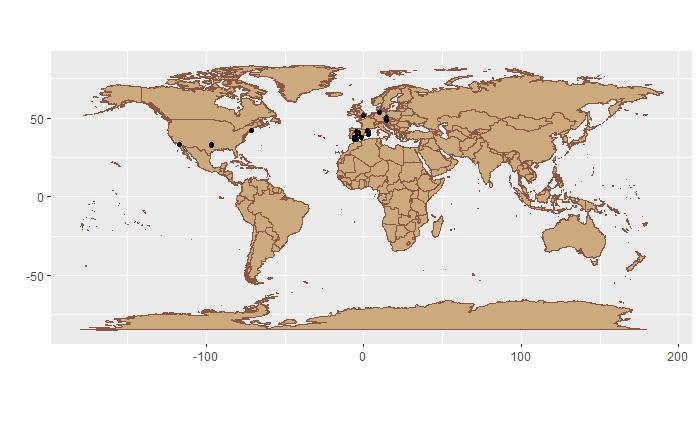
\includegraphics[scale=0.8]{img/madrid.jpg}  %el parámetro scale permite agrandar o achicar la imagen. En el nombre de archivo puede especificar directorios
\label{img/madrid.jpg}
\caption{Avistamientos Madrid}
\end{figure}

Es decir hay puntos en Madrid que no están situados en el mapa en una posición cercana a Madrid. En un principio pensamos que esto se debía a que el sistema de coordenadas del mapa sobre el que dibujamos los puntos, y los de la longitud y la latitud de nuestro dataset no coincidían. Pero antes de tomar una decisión sobre estos atributos decidimos dibujar los avistamientos relativos a pokemon que sólo aparecen en una regiones exclusivas: Mr. Mime en Europa, Tauros en Norte América, Kangaskhan en Australasia y Farfetch'd en Asia:

\begin{figure}[H] %con el [H] le obligamos a situar aquí la figura
\centering
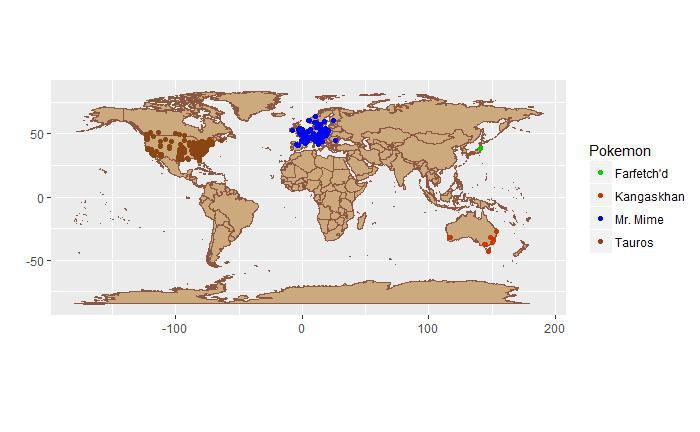
\includegraphics[scale=0.8]{img/exclusivos.jpg}  %el parámetro scale permite agrandar o achicar la imagen. En el nombre de archivo puede especificar directorios
\label{img/exclusivos.jpg}
\caption{Avistamientos regiones exclusivas}
\end{figure}

Como podemos ver la localización de estas visualizaciones es correcta, por lo tanto consideramos que las descripción del creador del dataset del atributo \textbf{city} no es correcta  \textbf\textit{the city of a sighting}. Así que o bien este atributo es la ciudad del usuario que vio el pokemon o el uso de proxys (que muchos usuarios emplearon para falsificar su posición y así poder acceder a pokemon de otras localizaciones distintas a la suya real) ha falseado los datos. En cualquiera de los casos esta información no es de utilidad para la predicción que queremos realizar, con lo que la eliminamos, junto con el atributo\textbf{continent}.\\

Pero antes tratas de darle una utilidad a esta información. Y es que un dataset no sirve únicamente para el problema que se plantea con él. Al tener datos de una aplicación empleada por tantos usuarios internacionalmente el número de datos indirectos que podemos extraer de él es muy grande, y de gran utilidad. En esta ocasión, considerando que el atributo \textbf{city} se refiere a la ciudad del usuario y que por tanto la localización de las observaciones se debe a viajes reales realizados por los usuarios, podemos extraer información sobre los desplazamientos realizados por los usuarios de la aplicación. Aquí vemos los viajes realizados por habitantes de Oslo:

\begin{figure}[H] %con el [H] le obligamos a situar aquí la figura
\centering
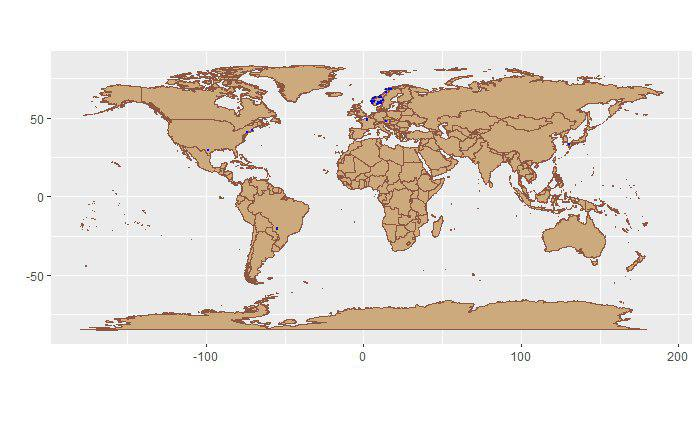
\includegraphics[scale=0.8]{img/oslo.jpg}  %el parámetro scale permite agrandar o achicar la imagen. En el nombre de archivo puede especificar directorios
\label{img/oslo.jpg}
\caption{Viajes realizados por los habitantes de Oslo}
\end{figure} 

En relación a estos datos indirectos que podemos obtener a partir de nuestro dataset podemos obtener también un mapa de temperaturas en el que se muestren las temperaturas en los lugares de los avistamientos. Como veremos más adelante los datos son relativos a una semana de agosto con lo que mostramos la temperatura referente a todos los avistamientos del dataset en un mismo mapa:

\begin{figure}[H] %con el [H] le obligamos a situar aquí la figura
\centering
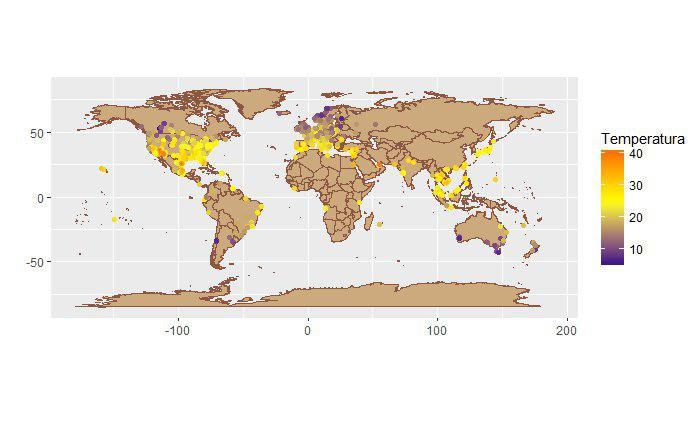
\includegraphics[scale=0.8]{img/temperatura.jpg}  %el parámetro scale permite agrandar o achicar la imagen. En el nombre de archivo puede especificar directorios
\label{img/temperatura.jpg}
\caption{Temperatura de los avistamientos}
\end{figure}

Aquí podemos apreciar por ejemplo como en Argentina las temperaturas son bajas en agosto, y como hay una diferencia de temperatura entre el norte y el sur de Europa.\\

Por otro lado al explorar el dataset observamos que en el atributo \textbf{appearedDayOfWeek} se tomaba el valor \textbf{dummy\_day}, y al consultar los valores que toma este atributo a lo largo del dataset vimos que no aparecía el lunes cuando el resto de los días de la semana sí que aparecen, con lo cual procedimos a revisar si este valor del atributo se corresponde con el lunes o es simplemente un valor perdido.\\

Observamos que el único día en el que se registran observaciones en las que el atributo toma el valor dummy\_day es el 8 de agosto, un lunes. Además, mientras se comprobaba este hecho observamos que todas las observaciones se realizaron en agosto y que además fue durante una semana de agosto, con lo cual el atributo \textbf{appearedMonth} no aporta ninguna información y además los atributos \textbf{appearedDayOfWeek} y \textbf{appearedDay} aportan la misma información, ya que al tomarse las muestras durante una sola semana hay una correspondencia biyectiva entre los valores de ambos atributos. Y como a priori no consideramos que la distancia entre días sea significativa, optamos por quedarnos con el atributo categórico.\\

Comprobamos también que podemos obtener los atributos sunriseMinutesMidnight y sunsetMinutesMidnight a partir de los atributos: \textbf{sunriseHour}, \textbf{sunriseMinute}, \textbf{sunsetHour} y \textbf{sunsetMinute}, con lo que procedemos a eliminar estos 4 últimos.\\

Veamos entonces cómo se distribuyen las muestras que tenemos según el tipo de pokemon avistado:

\begin{figure}[H] %con el [H] le obligamos a situar aquí la figura
\centering
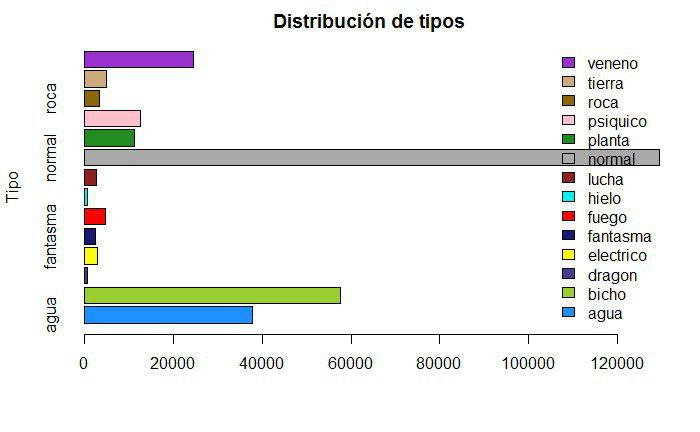
\includegraphics[scale=0.8]{img/tipos.jpg}  %el parámetro scale permite agrandar o achicar la imagen. En el nombre de archivo puede especificar directorios
\label{img/tipos.jpg}
\caption{Distribución de los tipos}
\end{figure}

Como podemos ver una vez que hemos agrupado las muestras por el tipo de pokemon, las clases están tremendamente desequilibradas. Mientras que hay muchísimos avistamientos de Pokemon de tipo normal, las clases hielo, dragón, fastasma, eléctrico o roca resultan marginales.\\

Creíamos que íbamos a apreciar una tendencia en la que los pokemon de tipo fantasma fuesen los que apareciesen con mayor frecuencia durante la noche, sin embargo todos los tipos siguen este patrón de aparición:

\begin{figure}[H] %con el [H] le obligamos a situar aquí la figura
\centering
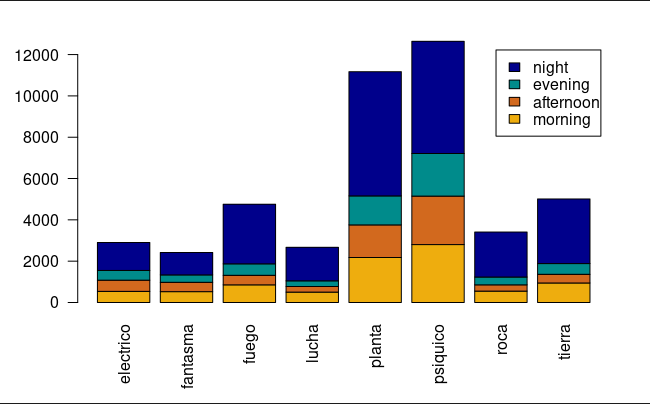
\includegraphics[scale=0.8]{img/noche1.png}  %el parámetro scale permite agrandar o achicar la imagen. En el nombre de archivo puede especificar directorios
\label{img/noche1.jpg}
\caption{Distribución de avistamientos a lo largo del día}
\end{figure}

\begin{figure}[H] %con el [H] le obligamos a situar aquí la figura
\centering
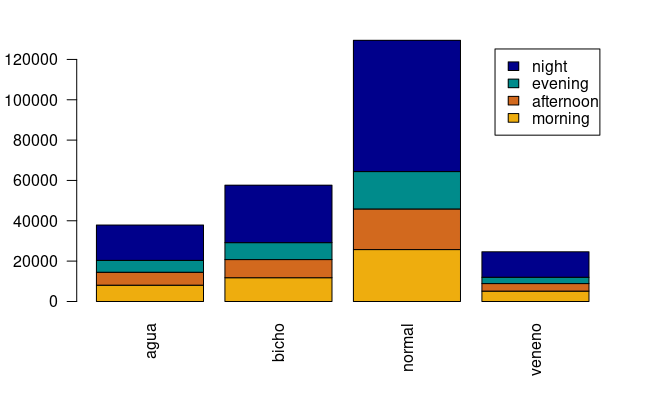
\includegraphics[scale=0.8]{img/noche2.png}  %el parámetro scale permite agrandar o achicar la imagen. En el nombre de archivo puede especificar dire2ctorios
\label{img/noche2.jpg}
\caption{Distribución de avistamientos a lo largo del día}
\end{figure}

\begin{figure}[H] %con el [H] le obligamos a situar aquí la figura
\centering
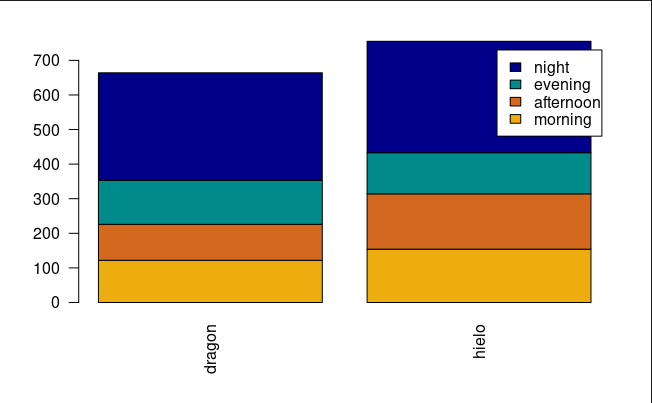
\includegraphics[scale=0.8]{img/noche3.png}  %el parámetro scale permite agrandar o achicar la imagen. En el nombre de archivo puede especificar directorios
\label{img/noche3.jpg}
\caption{Distribución de avistamientos a lo largo del día}
\end{figure}

Una de las principales características de Pokemon GO, aplicación de la cual son estos datos, es la posibilidad de encontrar pokemon en cualquier parte, por ejemplo en entornos cercanos al agua. Esperábamos, como es natural, que la mayoría de pokemon tipo agua se encuentren en zonas cercanas al agua. Esto daría un gran grado de realismo a la aplicación. Para comprobar esto generamos la siguiente gráfica:

\begin{figure}[H] %con el [H] le obligamos a situar aquí la figura
\centering
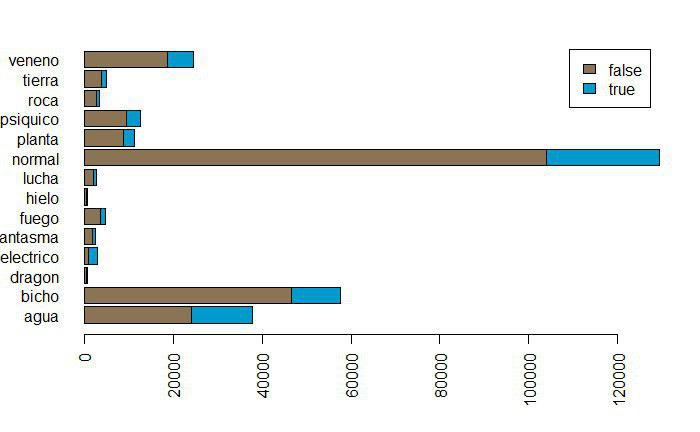
\includegraphics[scale=0.8]{img/cercaagua.jpg}  %el parámetro scale permite agrandar o achicar la imagen. En el nombre de archivo puede especificar directorios
\label{img/cercaagua.jpg}
\caption{Avistamientos cerca del agua}
\end{figure}

Así vimos que los pokemon de tipo eléctrico, dragón, agua e hielo son los que aparecen en mayor proporción cerca del agua. Por otro lado los pokemon de tipo fuego, planta, roca, normal y bicho son los que en menor proporción se presentan en zona acuosas (obtuvimos también una tabla para ver estos datos en cifras y no sólo visualmente). Nos sorprende de este análisis dos cosas: que no sean los pokemon de tipo agua los que sean más habituales en proporción en zonas acuosas y que los pokemon de tipo planta estén en menor proporción en las zonas con agua que en las zonas secas.\\

Aquí estamos hablando de proporciones, si nos fijamos en cantidades sí son los pokemon (después de los normales) de tipo agua los que aparecen más veces cerca del agua, no obstante preferimos atender a las proporciones ya que no queremos tener en cuenta que hay unos tipo de pokemon más difíciles de encontrar que otros.\\

Antes hemos estado discutiendo sobre los días de las apariciones de los diferentes pokemon. Por lo que ahora vamos a ver cómo se distribuyen dichas apariciones a lo largo de los días de la semana.

\begin{figure}[H] %con el [H] le obligamos a situar aquí la figura
\centering
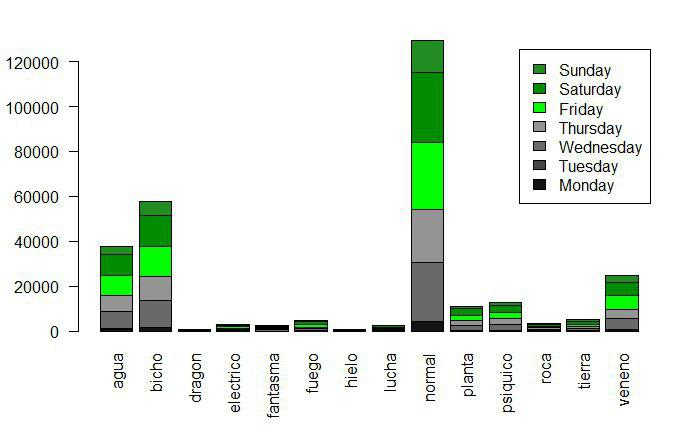
\includegraphics[scale=0.8]{img/semana.jpg}  %el parámetro scale permite agrandar o achicar la imagen. En el nombre de archivo puede especificar directorios
\label{img/semana.jpg}
\caption{Avistamientos a lo largo de la semana}
\end{figure}

Podemos observar que una gran parte de los avistamientos se realizan en el fin de semana, concretamente los sábados y viernes. También se producen una gran cantidad de avistamientos los miércoles y jueves, mientras que el lunes es el día que menos avistamientos se producen. Todo puede tener sentido, hemos de pensar que los datos que estamos tratando son de un vídeo juego para móviles, por lo tanto la mayor actividad, avistamientos, se realizará cuando los jugadores dispongan de mayor tiempo libre para jugar, fin de semana.\\

Ahora vamos a ver cómo se distribuyen los tipos de los distintos pokemon avistados en el mundo.

\begin{figure}[H] %con el [H] le obligamos a situar aquí la figura
\centering
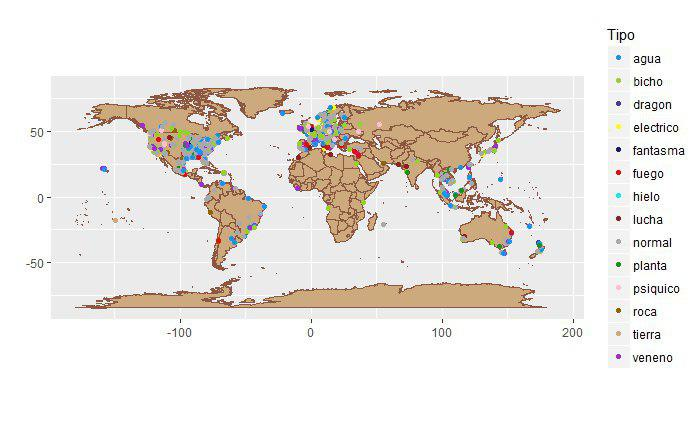
\includegraphics[scale=0.8]{img/tiposmundo.jpg}  %el parámetro scale permite agrandar o achicar la imagen. En el nombre de archivo puede especificar directorios
\label{img/tiposmundo.jpg}
\caption{Tipos de pokemon a lo largo del mundo}
\end{figure}

Podemos ver cómo no se sigue ningún tipo de distribución fija, no podemos obtener ningún tipo de patrón atendiendo a estos datos, por lo que se puede decir que los tipos de pokemon que aparecen son aleatorios.\\

Siguiendo esta línea estudiamos cómo se distrubuyen los tipos según la dirección e intensidad del viento:

\begin{figure}[H] %con el [H] le obligamos a situar aquí la figura
\centering
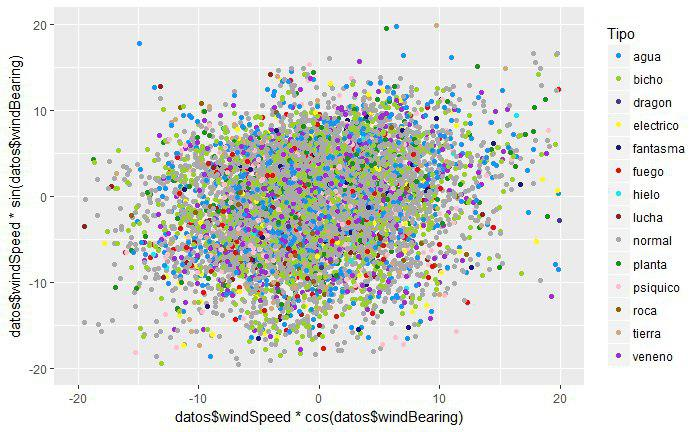
\includegraphics[scale=0.8]{img/viento.jpg}  %el parámetro scale permite agrandar o achicar la imagen. En el nombre de archivo puede especificar directorios
\label{img/viento.jpg}
\caption{Distribución de tipos según intensidad y dirección de viento}
\end{figure}

Aunque viendo los tipos uno por uno podríamos observar alguna tendencia hacia alguno de los cuadrantes de direcciones de viento lo cierto es que no hay una tendencia clara y podemos encontrar observaciones de cualquier tipo en cualquier dirección y velocidad, la densidad de puntos es mayor para velocidades menores pero para cualquier tipo se da la misma tónica. De hecho nos hemos restringido a una área más reducida para apreciar alguna tendencia y no hemos observado nada destacable.

\section{Clasificación}

Debido a que tenemos un dataset con un número tan grande de datos, para poder enfrentarnos a un problema de clasificación hemos decidido quedarnos con las muestras del dataset relativas a avistamientos de 5 especies de pokemon (Exeggcute, Squirtle, Pinsir, Meowth y Kakuna). No hemos optado por quedarnos con muestras relativas a 5 tipos de pokemon ya que, por un lado el número de datos seguiría siendo demasiado grande para tratarlo computacionalmete, y por otro consideramos que los datos relativos a las muestras de una especie de pokemon serían más homogéneos que aquellos relativos a un tipo de pokemon concreto. Optamos por estas especies ya que tienen un número adecuado de muestras y no están demasiado desequilibradas, aunque como veremo más adelante estas medidas no han sido especialmente efectivas de cara a los resultados de la clasificación.\\

Una vez hemos elegido el subconjunto de datos sobre el que trabajaremos vamos a realizar un proceso de preprocesamiento sobre este conjunto para poder hacerlo operativo de cara a los métodos de clasificación que emplearemos. Así, en primer lugar eliminamos los atributos \textbf{pokemonId} y \textbf{class} ya que esta información es justamente la que intentamos predecir con los distintos algoritmos que probaremos. Por otro lado también eliminamos el \textbf{tipo} del pokemon; este tipo se deduce directamente de la clase del pokemon con lo que no obtendríamos unos resultados de clasificación reales si lo dejásemos en el nuevo dataset.\\

A continuación limpiamos el dataset eliminando aquellos atributos que sólo presenten un valor a lo largo de todas las muestras, estos atributos no aportarán ninguna información al proceso de clasificación.\\

En un primer uso del dataset para probar los árboles de decisión nos encontramos con que una variable factor tenía más de 32 niveles con lo que los árboles no podían trabajar con nuestro dataset. Al revisar los tipos de variable del dataset nos encontramos con la el atributo \textbf{pokestopDistanceKm} era de tipo factor. Esto no tiene sentido ya que realmente esta variable es simplemente una variable que nos da la distancia en kilómetros del avistamiento de un pokemon a una poke-parada. Por lo tanto pasamos esta variable a numérica.\\

Al pasar esta variable a numérica observmos que teníamos valores perdidos en nuestro dataset, algo que se nos había pasado por alto anteriomente. Pasamos entonces a revisar si nuestro dataset buscando valores perdido, dado que sólo teníamos una muestra que presentase un valor perdido decidimos eliminarla del dataset simplemente.\\

Además, dado a que vamos a hacer uso de algoritmos como el KNN que dependen de la distancia entre las distintas muestras, antes de pasar a emplear estos algoritmos vamos a realizar una normalización de las variables al intervalo [0,1]. Por esta misma razón pasamos aquellos atributos categóricos de dos niveles (que son 1 y 2) a variables numéricas con valores 0 y 1. Estros atributos son los relativos a las coocurrencias y el \textbf{closeToWater}.\\

Nuevamente debido a la influencia de la distancia pasamos los atributos categóricos con más de 2 niveles  a atributos binarios, uno por cada nivel de cada uno de estos atributos. Por otro lado al intentar usar la función tree para obtener un árbol de decisión obtuvimos un error diciendo que teníamos una variable categórica con más de 32 nivels, observamos que el atributo \textbf{pokestopDistanceKm} era categórico, algo que no consideramos que tenga mucho sentido. Con lo cual pasamos a transformar este atributo a numérico. 

Con el dataset con esta configuración pasamos a aplicar y probar diversos algoritmos de clasificación sobre nuestro dataset. Para ello elaboramos una partición de train y otra de test (80-20) empleando la función \code{createDataPartition} del paquete \code{caret} que tiene la ventaja de que elabora estas particiones manteniendo la proporción entre las distintas especies del dataset. Obtuvimos así los siguientes resultados:

\begin{table}[H]
\centering
\caption{Resultados de clasificación}
\label{my-label}
\begin{tabular}{|l|c|}
\hline
\rowcolor[HTML]{FFFC9E} 
\multicolumn{1}{|c|}{\cellcolor[HTML]{FFFC9E}\textbf{Algoritmo}} & \textbf{Tasa de acierto en test} \\ \hline
tree                                                             & 34.12\%                          \\ \hline
ctree                                                            & 39.53\%                          \\ \hline
rpart                                                            & 38.43\%                          \\ \hline
KNN (k = 9)                                                      & 34.12\%                          \\ \hline
random forest                                                    & 44.75\%                          \\ \hline
xgboost                                                          & 45.90\%                          \\ \hline
\end{tabular}
\end{table}

En primer lugar hemos empleado árboles de decisión, en concreto hemos probado 3 algoritmos distintos para construir árboles de decisión, el que mejor resultado a obtenido ha sido \textbf{ctree}.

\begin{figure}[H]
	\centering
	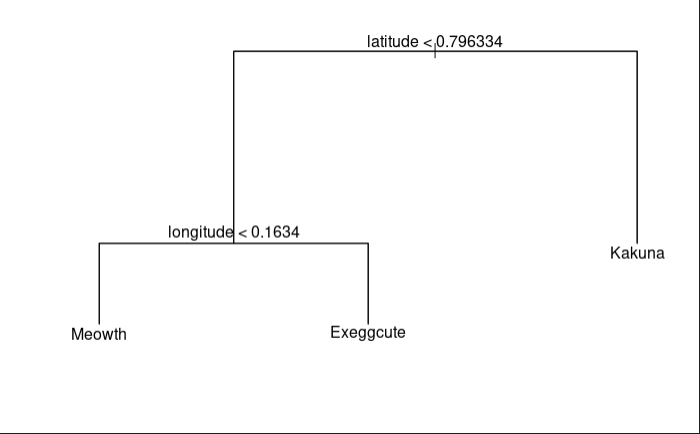
\includegraphics[width=\textwidth]{img/tree.png}
	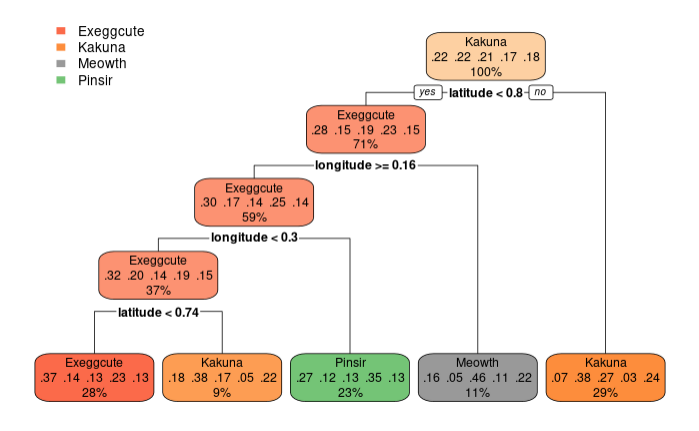
\includegraphics[width=\textwidth]{img/rpart.png}
\end{figure}

En las capturas anteriores podemos ver cómo los atributos empleados por dos de los 3 árboles de decisión construidos son \textbf{latitude} y \textbf{longitude}, de hecho observaremos esta tendencia en otro algoritmo más adelante. Pese a que rpart consigue una partición de los elementos del conjunto de train dando lugar a al menos un nodo hoja para cada una de las especies de pokemon que tenemos, no obtenemos un buen resultado de clasificación en test.\\

Para knn empleamos k = 9 ya que en una ejecución de la función \code{tune.knn} (probablemente sobre un dataset distinto al que finalmente empleamos en clasificación) obtuvimos que le mejor k precisamente 9. Si ejecutamos esta función sobre el conjunto actual obtenemos que el mejor k es 1, indicando posiblemente que las distintas clases están muy solapadas unas con otras en el dataset. Si bien es cierto que con k igual a 9 obtenemos un resultado ligeramente superior a emplear k = 1 (32.72\%).\\

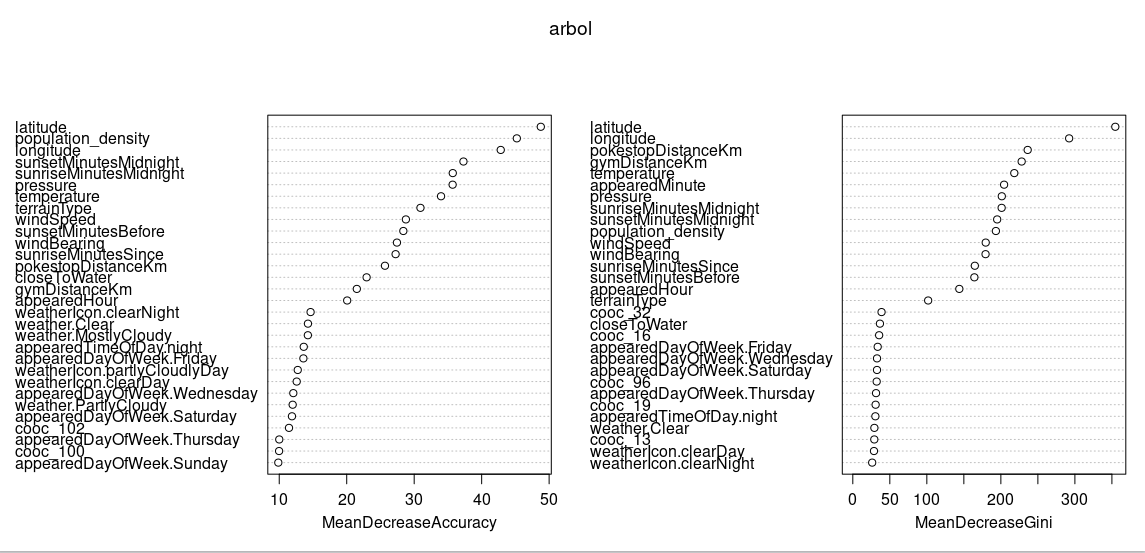
\includegraphics[width=\textwidth]{img/importancia.png}

En la gráfica anterior podemos ver cómo la longitud y la latitud vuelven a ser atributos muy determinantes para la clasificacion de los árboles de random forest, pese a que no se han obtenido tampoco unos resultados buenos en la clasificación. Tratamos, dado que estos atributos parecían tan importantes, a imponer a xgboost que sólo pudiese obtener árboles con un máximo de profundidad 2 para forzarlo a sólo usar estos dos atributos, los resultados empeoraron (ya hemos visto cómo se producen árboles de decisión más profundos usando sólo estos dos atributos en rpart).\\
 
Acabamos este estudio sobre los resultados de clasificación obtenidos haciendo una observación propia que probablemente sea errónea pero no obstante consideramos que es interesante incluirla en nuestro trabajo: el error que se puede producir en la clasificación se puede descomponer en dos componentes, el bias (la diferencia que hay entre el valor real a predecir y el predicho) y la varianza (erro debido al propio ruido del dataset). Encontrar un algoritmo que minimice ambos tipo de error simultáneamente es muy complicado y cada uno de los dos algoritmos de \textit{ensamble} que hemos empleado se centran en reducir uno de los dos. Mientras que random forest combina árboles más complejos independiente unos de otros para reducir el bias, xgboost emplea árboles más simples (aunque nosotros podemos controlar la profundidad máxima de los árboles empleados) tratando así de reducir la varianza.\\

Entonces, dado que ninguno de los dos enfoques anteriores da un resultado mucho mejor que el otro, pensamos que el dataset puede que no tenga información errónea o con ruido, pero que en cambio esta información no parece ser suficiente o adecuada para poder realizar una buena clasificación.

\section{Reglas de asociación}

Pasamos ahora a ver qué resultados hemos obtenido a partir de las reglas de asociación encontradas sobre el dataset completo. A fin de poder obtener reglas con un tiempo de ejecución abordable optamos por buscar reglas de hasta tamaño 3 y con una confianza de 0.8.\\

Además dado que pretendíamos encontrar reglas que nos dijesen algo acerca del tipo o la especie del pokemon pasamos las reglas obtenidas a una tabla de modo que pudiésemos hacer búsquedas en esta tabla del tipo ``extrae reglas que en su consecuente tengan una igualdad implicando al tipo del pokemon y que en el antecedente no aparezca el nombre del pokemon''.\\

Aunque las reglas obtenidas tenían un lift igual o superior a uno no hemos encontrado ninguna regla que sea de interés. La única que cabría señalar sería que con un 0.8 de confianza podemos decir que los tipo bicho y normal no aparecen cerca del agua.\\

Por lo tanto, al igual que sucedía en clasificación, los resultados obtenidos sobre nuestro dataset no son de calidad.

\section{Conclusiones}

Veamos las conclusiones que extraemos de nuestro estudio tras todo este proceso:

\begin{enumerate}
\item La aplicación parece tener un mayor uso durante el fin de semana y el viernes.
\item Se producen más avistamientos de pokemon durante la noche (no sólo de pokemon de tipo fantasma como suponíamos en un inicio).
\item Hay muchos atributos en este dataset que parecen no aportar información. El creador del dataset además ha añadido más atributos de los que puede obtener directamente de la aplicación, esta información adicional tampoco parece ser de utilidad.
\item No hemos de centrarnos sólo en resolver el principal problema que plantea un dataset, en este caso la clasificación. Un dataset puede tener más utilidad que la de resolver el problema que plantea, por ejemplo en nuestro caso hemos aprovechado el extendido uso de esta aplicación para obtener un mapa de temperaturas para una semana de agosto.
\item Hay ocasiones en que la descripción que nos dan de un dataset puede no ser la correcta y tendremos que tratar de averiguar si los datos que se nos proporcionan son realmente lo que el creador del dataset dice que son.
\item A la luz de los resultados de la clasificación y de la extracción de reglas de asociación parece que los avistamiento de pokemon, al menos en las cinco especies que hemos escogido (aunque ya vimos que también se daba para el conjunto entero), tiene una componente aleatoria.
\end{enumerate}

En cuanto a esta última observación vamos a ver una serie de gráficas que parecen poner de manifiesto la aleatoriedad de los avistamientos:\\

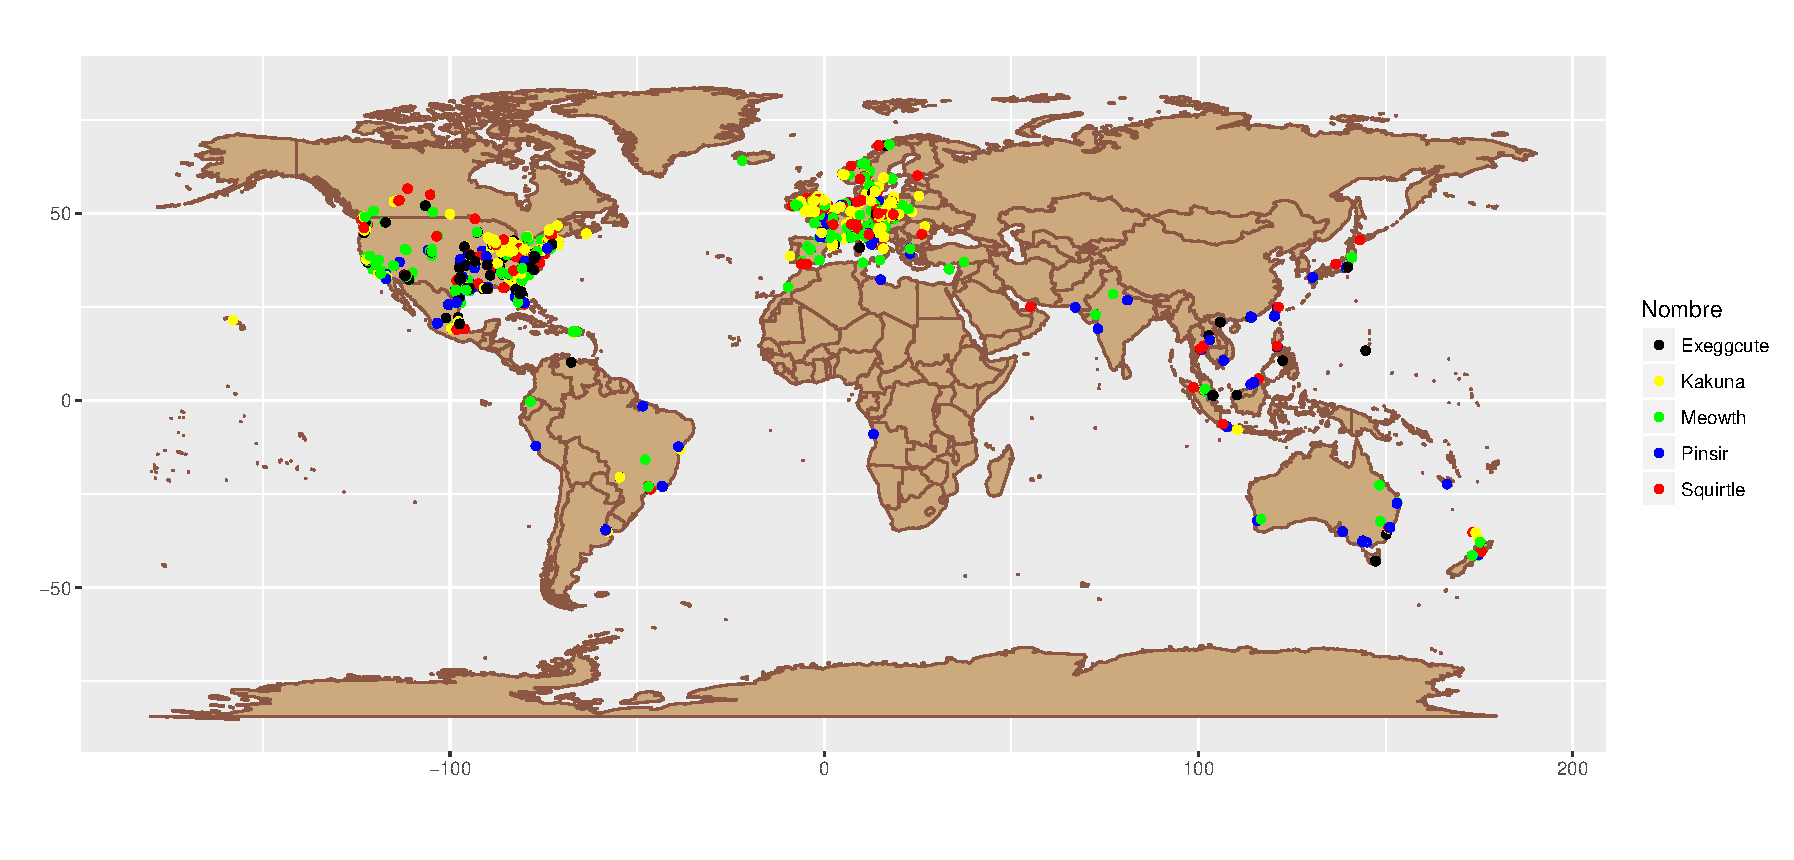
\includegraphics[width = \textwidth]{img/mapaFiltrado.pdf}

Aquí hemos mostrado los avistamiento de las 5 especies de pokemon escogidas. Hemos querido visualizar esto ya que como vimos random forest le daba mucha importancia a los atributos de latitud y longitud. Como podemos observar las 5 especies de pokemon escogidas están muy entremezcladas en el mapa, no pudiendo definir una región clara en la que sólo aparezca un tipo de especie.\\

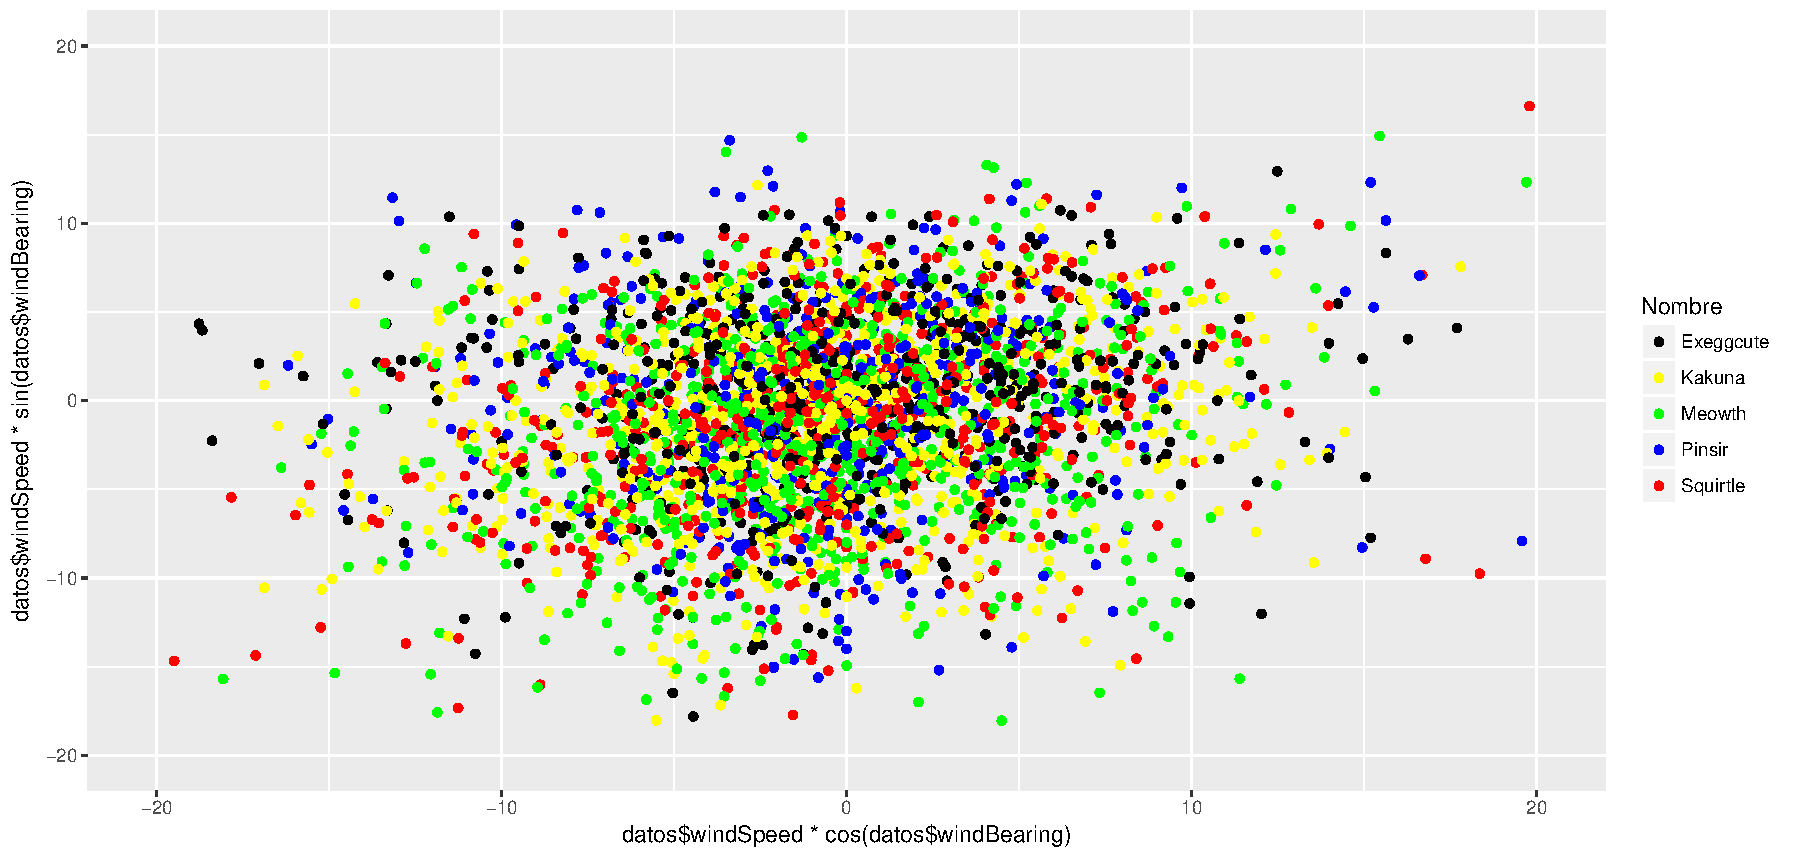
\includegraphics[width = \textwidth]{img/vientoFiltrado.pdf}

Al igual que hicimos para el dataset original hemos querido ver si había algún patrón en la velocidad y dirección del viento para cada una de las especies escogidas, como vemos los resultados han sido similares a los anteriores.

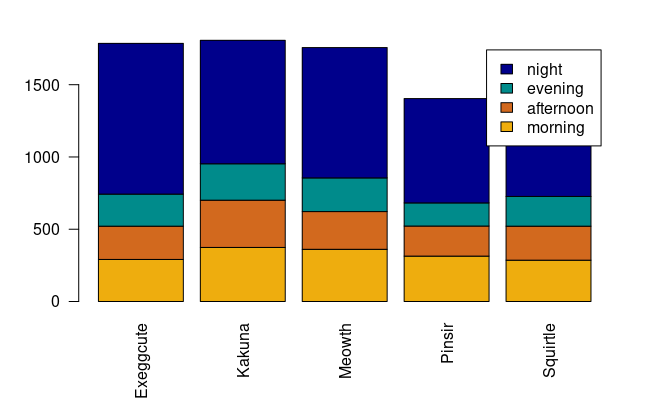
\includegraphics[width = \textwidth]{img/parteDiaFiltrado.png}

Por último aquí vemos, al igual que sucedía con los distintos tipos de pokemon, cómo los avistamientos de las distintas especies se distribuyen a lo largo de todo el día y no se concentran en una sólo parte del día. Con lo cual, a la luz de estas gráficas, no parece que decir que los avistamiento de pokemon tiene una componente aleatoria (al menos para las especies escogidas para hacer clasificación) sea una afirmación incorrecta.

\section{Material consultado}

\begin{itemize}
\item \href{https://www.kaggle.com/semioniy/predictemall}{El repositorio del dataset}.
\item Los scripts de R del material de la asignatura.
\item Algunos enlaces en los que se explicaba como elaborar algunas de las gráficas que hemos generado durante este estudio.
\end{itemize}

\end{document}